\documentclass[12pt]{article}

\setlength\parindent{0pt}
\newcommand{\myt}[1]{\textbf{\underline{#1}}}

\usepackage{mathtools}
\usepackage{amssymb}
\usepackage{graphicx}

\title{\vspace{-15ex}Math 239 Lecture 26\vspace{-1ex}}
\date{July 10th, 2015}
\author{Graham Cooper}

\begin{document}
	\maketitle
	
	\section*{Euler's Formula}
	
	Euler's formula for a planar embedding of a connected planar graph G with n vertices, m edges and S faces,\\
	$$n - m + S = 2$$
	
	\myt{Proof:} Fix the number of vertices n, do induction on the number of edges m.\\
	
	Base Case: m = n-1 (a tree, smallest connected planar graph)\\
	In a tree S = 1 So n - m + s = n - (n-1) + 1 = 2\\
	
	Induction Hypothesis: Assume any connected planar embedding with n vertices and m-1 edges satisfy Euler's formula\\
	
	Induction Step: Consider a connected planar emb. if a graph G with n vertices, m edges, s faces. Since G is not a tree, it contains a cycle. Let e be an edge in a cycle. Then G-e is connected (sicne e is not a bridge), planar, with m-1 eges.\\
	By Induction hypothesis, Euler's formula holds for G-e. The edge e has 2 different faces on both sides. In G-e, these two faces merge into 1 so G-e has S-1 faces. Using Euler's formular for G-e, n-(m-1)+(s-1) = 2. So n-m+s = 2 and Euler's formula hodls for G.\\
	
	\section*{Platonic Solids}
	Any planar embedding can bedrawn on the sphere, cut off the faces to obtain a polyhedron.
	
	\myt{Definition} A connected graph is \underline{platonic} if it has an embedding where every verte has the same degree ($\geq$ 3)\\
	
	Suppose a platonic graph has n verices, m edges, s faces, $d_v \geq 3$ verte deg, $d_f \geq 3$ face deg\\
	
	\begin{enumerate}
		\item Handshaking lemma: 2m = n$\cdot d_v$ $\implies$ n = $\frac{2m}{d_v}$
		\item Handshaking lemma for faces: 2m = S $\cdot d_f$ $\implies$ S = $\frac{2m}{d_f}$
		\item Euler's Formula: n - m + s = 2\\
		$$\implies \frac{2m}{d_v} - m + \frac{2m}{d_f} = 2$$
		multiply by $d_vd_f$\\
		$$\implies 2md_f - md_vd_f + 2md_v = 2d_vd_f$$
		$$\implies m(2d_f - d_vd_f + 2d_v) = 2d_vd_f$$
		$$\implies 2d_f - d_vd_f + 2d_v > 0$$
		$$\implies 2d_f - d_vd_f + 2d_v - 4 + 4$$
		$$ = -(d_v - 2)(d_f - 2) + 4 > 0$$
		$$\implies (d_v - 2)(d_f - 2) < 4$$
	\end{enumerate}
	
	\begin{tabular}{c | c }
		$d_v$ & $d_f$ \\ \hline
		3 & 3,4,5 \\
		4 & 3 \\
		5 & 3 \\
	\end{tabular}
	
	Only possible \\
	$(d_v,d_f)$ pairs, $d_v = 3$ $d_f = 3$\\
	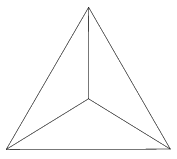
\includegraphics[scale=0.5]{tetrahedron.png}\\
	
	$d_v = 3$ $d_f = 4$\\
	
\includegraphics[scale=0.5]{cube.png}\\
	
	$d_v = 4$ $d_f = 3$\\
	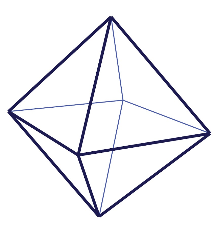
\includegraphics[scale=0.5]{octo.png}\\
	
\end{document}
